% Capíulo 4
\chapter{Avaliação} \label{ch:avaliacao}

Este capítulo descreve o estudo empírico realizado em dois sistemas \textit{open-source} de diferentes domínios cujos objetivos são avaliar se as visualizações são úteis para representar os desvios de desempenho encontrados durante a análise desses sistemas, avaliar se os usuários conseguem encontrar as informações sobre os desvios através das visualizações oferecidas e a verificar a possível aplicabilidade da ferramenta como parte integrande dos processos de desenvolvimento dos sistemas analisados.

O restante deste capítulo está organizado como segue: seção \ref{sec:avaliacao-projeto} apresenta como o estudo foi projetado, incluindo os objetivos e questões de pesquisa (subseção \ref{subsec:avaliacao-objetivos-questoes-pesquisa}), os sistemas analisados (subseção \ref{subsec:avaliacao-sistemas}) e os procedimentos do estudo (subseção \ref{subsec:avaliacao-procedimentos}); a seção \ref{sec:avaliacao-resultados} exibe os resultados do estudo e a seção \ref{sec:avaliacao-consideracoes} conclui o capítulo, apresentando as principais contribuições do estudo, as ameaças à validade e as limitações da avaliação aplicada.

\section{Projeto} \label{sec:avaliacao-projeto}

O estudo analisou um total de 20 releases dos projetos Jetty \cite{Jetty2016} e VRaptor \cite{VRaptor2017}, sendo 10 releases para cada sistema, considerando 193 cenários distintos ao total, gerando as visualizações de sumarização dos cenários e grafo de chamadas para todos os casos. Sobre as visualizações, foram coletados feedback de usuários desses sistemas através de um questionário online.

De maneira geral, foram aplicadas as fases discutidas no capítulo \ref{ch:pqae}, subseção \ref{subsec:funcionamento-perfminer}, além do procedimento necessário para gerar os dados para as visualizações, conforme descrito na seção \ref{sec:visao-geral-architecture-qa-evolution} do mesmo capítulo. Em suma: (i) primeiro, os casos de testes automatizados (cada um deles representando um cenário) dos sistemas foram executados e monitorados, resultando em múltiplos bancos de dados; (ii) depois, os dados coletados foram comparados, agrupando releases subsequentes para cada sistema; (iii) então, os elementos identificados com desvios de desempenho foram minerados nos seus sistemas de controle de versão, com o intuito de descobrir os \textit{commits} que alteraram esses artefatos; (iv) por fim, foi executado, para cada versão de cada sistema, o procedimento necessário para gerar os dados que dão suporte às visualizações. Após isso, o questionário online foi elaborado e aplicado.

O questionário foi enviado para todos os contribuidores no GitHub dos sistemas que possuiam endereço de email registrado na página de contribuidores de cada sistema ou na página do seu perfil. Dos 114 contribuidores que receberam o questionário, 16 deles responderam com algum feedback.

\subsection{Objetivos e Questões de Pesquisa} \label{subsec:avaliacao-objetivos-questoes-pesquisa}

Os principais objetivos deste estudo são investigar se a ferramenta \textit{\toolName}, com suas visualizações e propriedades visuais oferecidas, é capaz de representar as evoluções de desempenho dos cenários analisados, se os usuários conseguem identificar esses desvios através das representações visuais oferecidas e se é útil para as equipes de desenvolvimento dos sistemas analisados. Ao utilizar a ferramenta, os usuários poderão identificar os cenários com desvios de desempenho e, a partir da análise do grafo de chamadas de cada um deles, tomar conhecimento sobre os \textit{commits} dos métodos que possivelmente foram os responsáveis pelo desvio. A partir de então, ações podem ser tomadas pela equipe de desenvolvimento para sanar possíveis problemas no desempenho das aplicações. O estudo foi guiado pelas seguintes questões de pesquisa:

{\color{red}DESENVOLVER TEXTOS PARA AS QPS.}

\textbf{QP1: Os cenários identificados com desvios de desempenho são apresentados claramente nas visualizações implementadas pela ferramenta?}

\textbf{QP2. O algoritmo de redução de nós aplicado pela ferramenta é capaz de reduzir significativamente o número de nós no grafo de chamadas para sistemas reais?}

\textbf{QP3: Desenvolvedores e arquitetos conseguem identificar os cenários com variações de desempenho e suas potenciais causas, em termos de métodos e \textit{commits}, através do auxílio visual da ferramenta?}

\textbf{QP4: Há indícios de que as visualizações implementadas pela ferramenta são mais eficazes do que os dados tabulares para se encontrar informações sobre os cenários, métodos e \textit{commits}?}

\subsection{Sistemas} \label{subsec:avaliacao-sistemas}

Neste estudo foram usados dois sistemas \textit{open-source} de diferentes domínios selecionados através dos seguintes critérios:
\begin{itemize}
  \item Ser desenvolvido na linguagem de programação Java;
  \item Ter no mínimo dez releases (no momento do início do estudo);
  \item Possuir casos de testes automatizados utilizando a biblioteca JUnit;
  \item Estar listado em uma das categorias do site \href{http://java-source.com}{http://java-source.com} (site de projetos \textit{open-source} em Java). Os sistemas foram escolhidos de modo que não houvesse repetição de categorias;
  \item Possuir repositório no GitHub.
\end{itemize}

A partir desses critérios, foram escolhidos os sistemas Jetty \cite{Jetty2016} e o VRaptor \cite{VRaptor2017}. O Jetty é um servidor web e um servlet contêiner Java capaz de fornecer conteúdo estático e dinâmico a partir de instanciações \textit{standalone} ou embutidas. As dez últimas releases do Jetty foram 9.3.10, 9.3.11, 9.3.12, 9.3.13, 9.3.14, 9.3.15, 9.3.16, 9.4.0, 9.4.1 e 9.4.2.

O VRaptor é um \textit{framework} MVC para desenvolvimento web em Java que visa trazer alta produtividade para um desenvolvimento com CDI \abrv[CDI -- \textit{Contexts and Dependency Injection}]{(\textit{Contexts and Dependency Injection}).} As dez últimas releases do VRaptor foram 4.0.0.Final, 4.1.0.Final, 4.1.1, 4.1.2, 4.1.3, 4.1.4, 4.2.0.RC1, 4.2.0.RC2, 4.2.0.RC3 e 4.2.0.RC4.

\subsection{Procedimentos} \label{subsec:avaliacao-procedimentos}

Esta subseção descreve os procedimentos seguidos após a escolha dos sistemas, organizados sequencialmente nos passos a seguir.

\subsubsection{Passo 1 - Coleta e Preparação dos Dados} \label{subsec:avaliacao-procedimentos-passo-1}

Após a escolha dos sistemas e suas releases, os códigos-fonte de todas elas foram baixadas do repositório com a finalidade de executar as três fases do \textit{\perfMinerName}. Após o download, cada uma das versões foi configurada para compilar e executar sem erros, uma vez que a fase 1 necessita exercitar a aplicação através dos testes automatizados. Todos os testes executados são considerados como pontos de entrada de cenários. Para o cálculo do desvio de desempenho, o \textit{\perfMinerName} não considera quaisquer desvios a partir de classes de teste, somente de classes do código-fonte da aplicação.

De posse dos códigos-fonte, cada release dos projetos foi configurada para dar suporte ao \textit{AspectJ} e para incluir as bibliotecas do \textit{\perfMinerName}, no entanto, de maneira não intrusiva, sem qualquer alteração no código-fonte.

\subsubsection{Passo 2 - Aplicação da Abordagem} \label{subsec:avaliacao-procedimentos-passo-2}

Após isso, para cada versão de cada sistema, todos os casos de testes automatizados foram executados para que os dados da análise dinâmica (fase 1) fossem coletados pela ferramenta.

A análise dinâmica para todas as releases foi executada no mesmo computador sob as mesmas condições e com serviços não essenciais desabilitados. A configuração do computador utilizado foi um AMD Phenom II com 8 GB de memória RAM, executando o sistema operacional Linux Ubuntu 16.04 LTS e o Java na versão 8. A suite de testes automatizados de cada release foi executada dez vezes nas mesmas condições a fim de obter médias de desempenho, em termos de tempo de execução, mais precisas.

Na sequência, as dez releases de cada sistema foram agrupadas em 9 pares de evoluções para executar as fases 2 e 3 do \textit{\perfMinerName}, além da extensão proposta pelo \textit{\toolName}. A tabela \ref{tab:summary-releases-jetty-vraptor} a seguir mostra como ficaram organizados esses pares para cada sistema.

\begin{table}[!htb]
  \textsf{\caption{Organização dos pares de releases para o Jetty e VRaptor.\label{tab:summary-releases-jetty-vraptor}}}
  \centering
  \medskip
  \begin{tabular}{c|c|c|c}
  \multicolumn{2}{c|}{\textbf{Jetty}} & \multicolumn{2}{c}{\textbf{VRaptor}} \\ \hline
  9.3.10 & 9.3.11 & 4.0.0.Final & 4.1.0.Final \\ \hline
  9.3.11 & 9.3.12 & 4.1.0.Final & 4.1.1 \\ \hline
  9.3.12 & 9.3.13 & 4.1.1 & 4.1.2 \\ \hline
  9.3.13 & 9.3.14 & 4.1.2 & 4.1.3 \\ \hline
  9.3.14 & 9.3.15 & 4.1.3 & 4.1.4 \\ \hline
  9.3.15 & 9.3.16 & 4.1.4 & 4.2.0.RC1 \\ \hline
  9.3.16 & 9.4.0 & 4.2.0.RC1 & 4.2.0.RC2 \\ \hline
  9.4.0 & 9.4.1 & 4.2.0.RC2 & 4.2.0.RC3 \\ \hline
  9.4.1 & 9.4.2 & 4.2.0.RC3 & 4.2.0.RC4 \\ \hline
  \end{tabular}
\end{table}

Na fase 2, o resultado da análise dinâmica para cada par de releases mostrado anteriormente foi recuperado e comparado, entre os pares, com a finalidade de determinar métodos e contrutores com degradação ou otimização de desempenho. Já na fase 3, os elementos com desvios de desempenho foram minerados nos seus sistemas de controle de versão e sistemas de gerenciamento de tarefas. Ao final das 3 fases do \textit{\perfMinerName}, são gerados os artefatos de saída requeridos para o \textit{\toolName}. Vale salientar neste ponto que, embora o \textit{\perfMinerName} relalize a mineração e obtenha o conjunto de tarefas que estão relacionadas com os \textit{commits} que possivelmente foram os responsáveis por inserir determinado desvio de desempenho, a integração com essas ferramentas de gerenciamento de tarefas está, até este momento, fora do escopo do \textit{\toolName}.

Com os artefatos de saída, a fase 4, pertencente à extensão proposta, foi iniciada. Para cada sistema e um par de releases foi executada a análise descrita na subseção \ref{subsec:new-analysis}, cuja finalidade é, a partir desses artefatos, realizar um processamento com o intuito de gerar os dados que dão suporte às visualizações. Após a execução dessa fase, iniciou-se o processo de verificação das visualizações geradas para, posteriormente, publicar o resultado das análises em um ambiente na nuvem, o Heroku\footnote{\href{http://www.heroku.com}{http://www.heroku.com}}, cujo endereço é \href{http://apvis.herokuapp.com}{http://apvis.herokuapp.com}.

\subsubsection{Passo 3 - Elaboração e Aplicação dos Questionários} \label{subsec:avaliacao-procedimentos-passo-3}

A elaboração do questionário se deu na sequência, após a publicação dos resultados das análises. O questionário foi dividido em 5 seções: (i) uma com questões demográficas, (ii) outra com questões sobre o atributo de qualidade de desempenho, (iii) uma terceira com questões sobre a visualização do grafo de chamadas, (iv) outra sobre a visualização da sumarização de cenários e, por fim, (v) uma seção com questões gerais que concluem o questionário. Todas as questões do questionário foram opcionais.

A primeira seção foi elaborada com o intuito de coletar informações sobre a experiência dos participantes no desenvolvimento de software na linguagem de programação Java e nos seus respectivos projetos. A segunda seção continha questões sobre a experiência de uso de ferramentas de \textit{profiling} e APM, e sobre estratégias que os participantes utilizam para gerenciar o desempenho das funcionalidades dos respectivos sistemas. Na terceira seção, foram perguntadas questões sobre a visualização do grafo de chamadas. Foram dadas situações para que eles se baseassem ao responderem as questões. Além disso, foi perguntado sobre os aspectos que eles mais e menos gostaram com relação a visualização. A mesma estratégia foi utilizada para a quarta seção do questionário, mas relacionada à visualização da sumarização de cenários. Na quinta e última seção, os participantes responderam sobre os benefícios de se utilizar a ferramenta, bem como se eles a usariam nos processos de desenvolvimento de software dos seus respectivos sistemas. Os participantes tiveram acesso a todos os resultados gerados pela ferramenta no final do questionário.

Os participantes foram agrupados de acordo com o sistema em que contribui. Sendo assim, dois grupos foram formados: 66 participantes para grupo de contribuidores Jetty e 48 para o grupo de contribuidores do VRaptor. Depois, cada grupo foi dividido em dois, de modo que, para cada sistema, foram aplicados dois tipos de questionários. A tabela \ref{tab:survey-groups} mostra a divisão dos grupos de participantes:

\begin{table}[!htb]
  \centering
  \textsf{\caption{Distribuição dos grupos de participantes.\label{tab:survey-groups}}}
  \medskip
  \begin{tabular}{c|c|c|c|c}
  \textbf{Grupo} & \textbf{Sistema} & \textbf{\begin{tabular}[c]{@{}c@{}}Quantidade\\ de Participantes\end{tabular}} & \textbf{\begin{tabular}[c]{@{}c@{}}Tipo de\\ Questionário\end{tabular}} & \textbf{Idioma} \\ \hline
  A & Jetty & 33 & Tipo 1 & Inglês \\ \hline
  B & Jetty & 33 & Tipo 2 & Inglês \\ \hline
  C & VRaptor & 24 & Tipo 1 & Português \\ \hline
  D & VRaptor & 24 & Tipo 2 & Português \\ \hline
  \end{tabular}
\end{table}

Os tipos dos questionários têm as seguintes características: 

\begin{itemize}
    \item \textit{Tipo 1}: neste tipo o participante respondeu às questões sobre a visualização do grafo de chamadas através da visualização exibida pela ferramenta. Por outro lado, as questões sobre a visualização da sumarização de cenários foram respondidas baseadas em resultados dispostos em uma tabela, ao invés da visualização fornecida pela ferramenta;
    \item \textit{Tipo 2}: é o inverso do anterior: o participante respondeu às questões sobre a visualização do grafo de chamadas se baseando em resultados exibidos em uma tabela e respondeu às questões sobre a visualização da sumarização de cenários através da visualização mostrada pela ferramenta.
\end{itemize}

A divisão do questionário nesses dois tipos permite que as respostas sejam comparadas entre os que responderam baseados nas visualizações da ferramenta e os que responderam baseados em dados tabulares. Ambos os tipos tiveram questões iguais, no entanto, utilizando referências específicas aos cenários dos projetos analisados, quando aplicado nas questões. Através dessa divisão, pode ser comparado, por exemplo, o porcentual de acerto às questões com e sem as visualizações. Além disso, as perguntas sobre as visualizações permitem coletar informações sobre a identificação correta de elementos, a facilidade de se identificar esses elementos e as impressões dos participantes sobre elas. Os dois tipos do questionário podem ser consultados no apêncice \ref{ch:apendice-a} e os dados tabulares usados pelos participantes pode ser encontrado no link \href{https://goo.gl/DJwtLT}{https://goo.gl/DJwtLT}.

Com o questionário elaborado, foram coletados os dados de email e login dos contribuidores de cada projeto através da API do Github. No entanto, não foi possível coletar esses dados para todos os contribuidores pelo fato de existir uma opção nessa ferramenta em que os usuários podem desabilitar a publicização do seu endereço de email nessa API. Para esses casos foram feitas visitas manuais aos perfis de cada contribuidor. Ao final desse processo, foram submetidos 66 questionários para os contribuidores do Jetty e 48 para os contribuidores do VRaptor, um total de 114.

\subsection{Caracterização dos Participantes} \label{subsec:avaliacao-caracterizacao-participantes}

Dos contribuidores que receberam o questionário, 16 deles responderam com algum feedback: 9 do Jetty e 7 do VRaptor, uma taxa de resposta de 14,04\%. Das respostas, 3 foram consideradas inválidas, pois: (i) em uma delas, o usuário abriu a ferramenta em um celular, comprometendo as visualizações e, consequentemente, as suas respostas; (ii) outro usuário, ao invés de abrir a ferramenta para responder às questões respondeu com base em apenas uma figura explicativa elaborada para elucidar informações sobre as visualizações; e (iii) o terceiro usuário respondeu apenas as questões demográficas, deixando todas as outras em branco. Portanto, 13 respostas foram consideradas válidas para a análise dos resultados.

A maioria dos participantes que responderam são desenvolvedores (31\%), arquitetos (15\%) e engenheiros (23\%) de software, possuem mais de 5 anos de experiência na linguagem de programação Java (figura \ref{fig:avaliacao-questao-2}) e possuem entre 1 e 10 contribuições no seu projeto (figura \ref{fig:avaliacao-questao-3}). Apesar de alguns participantes não terem contribuído para os projetos nos últimos 12 meses, o fato de serem experientes no desenvolvimento de software em Java podem dar credibilidade às suas respostas.

\begin{figure}[!htb]
  \centering
   \begin{subfigure}{.5\textwidth}
   \centering
   \frame{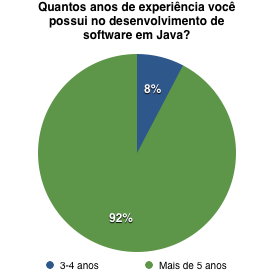
\includegraphics[scale=0.65]{Imagens/avaliacao_questao_2.png}}
   \textsf{\caption[Experiência.]{Experiência em desenvolvimento de software.\label{fig:avaliacao-questao-2}}}
   \end{subfigure}%
   \begin{subfigure}{.5\textwidth}
   \centering
   \frame{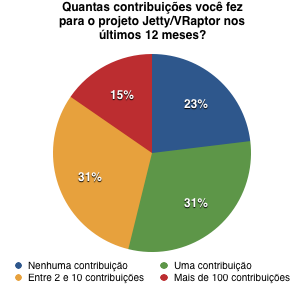
\includegraphics[scale=0.65]{Imagens/avaliacao_questao_3.png}}
   \textsf{\caption[Quantidade de contribuições.]{Quantidade de contribuições.\label{fig:avaliacao-questao-3}}}
   \end{subfigure}
   \caption{Dados demográficos dos participantes.}
  \label{fig:avaliacao-questoes-2-3}
\end{figure}

Sobre a experiência dos participantes com o uso de ferramentas de análise de desempenho, como ferramentas de \textit{profiling} ou ferramentas APM, 54\% declarou usar com frequência essas ferramentas e 15\% declarou já ter usado pelo menos uma vez. As ferramentas mais citadas pelos participantes foram: JProfiler, New Relic e JVisualVM.

Em resposta à questão \textit{``Suponha que uma funcionalidade do Jetty/VRaptor foi evoluída (por você ou outro membro da equipe). O que você faz para garantir que o tempo de execução/resposta de tal funcionalidade é aceitável em comparação com outras releases?''}, a maioria dos participantes respondeu que fazem a medição de desempenho, no entanto, foram várias as maneiras descritas por eles: o participante P4GA (participante 4 do grupo A) realiza a \textit{``medição e comparação de tempos de execução dos testes''}, já o participante P11GA menciona que faz o \textit{``teste de integração contínua de um teste de gerador de carga''}, o participante P13GC realiza \textit{``análise da complexidade do algoritmo envolvido na evolução e caso não seja possível garantir dessa forma, faço com alguns testes automatizados, seja unitário ou usando um software como o JMeter''} e o participante P6GD faz \textit{``comparação via NewRelic (response time - response time by endpoint - etc)''}.

\section{Resultados} \label{sec:avaliacao-resultados}

Nesta seção serão discutidos os resultados obtidos após a execução da ferramenta para os sistemas mencionados e após a aplicação do questionário online com os desenvolvedores dessas aplicações. A subseção \ref{subsec:avaliacao-comportamento-visualizacoes} comenta o comportamento das visualizações para os dados obtidos dos sistemas e a subseção \ref{subsec:avaliacao-questionario-online} apresenta os resultados obtidos após a aplicação do questionário.

\subsection{Análise do Comportamento das Visualizações} \label{subsec:avaliacao-comportamento-visualizacoes}

Após a execução dos passos 1 e 2 da subseção de Procedimentos (\ref{subsec:avaliacao-procedimentos}) foram verificadas as visualizações geradas e constatou-se que, de maneira geral, a representação visual dos dados analisados foi feita de maneira correta e safisfatória. As subseções seguintes apresentam os resultados da visualização de Sumarização de Cenários, mostrando exemplos em que a visualização foi gerada conforme esperado e outros que expõem situações onde a identificação dos cenários foi prejudicada, e da visualização do Grafo de Chamadas, expondo o algoritmo de supressão de nós exibidos além de comentar casos especiais ocorridos.

\subsubsection{Sumarização de Cenários} \label{subsec:avaliacao-comportamento-sumarizacao-cenarios}

Ao final da análise das releases selecionadas, foram encontrados um total de 244 cenários com desvios de desempenho, sejam degradações ou otimizações. Eles estão mostrados nas tabelas \ref{tab:summary-jetty} para o Jetty, e \ref{tab:summary-vraptor} para o VRaptor.

\begin{table}[!htb]
  \textsf{\caption{Resumo para o Jetty.\label{tab:summary-jetty}}}
  \centering
  \medskip
  \begin{tabular}{c|c|c|c|c}
  \textbf{Versão Inicial} & \textbf{Versão Final} & \textbf{\begin{tabular}[c]{@{}c@{}}Cenários\\ Degradados\end{tabular}} & \textbf{\begin{tabular}[c]{@{}c@{}}Cenários\\ Otimizados\end{tabular}} & \textbf{\begin{tabular}[c]{@{}c@{}}Total de\\ Cenários\end{tabular}} \\ \hline
  9.3.10 & 9.3.11 & 5 (3,18\%) & 1 (0,63\%) & 157 \\ \hline
  9.3.11 & 9.3.12 & 0 (0\%) & 36 (21,55\%) & 167 \\ \hline
  9.3.12 & 9.3.13 & 0 (0\%) & 7 (4,51\%) & 155 \\ \hline
  9.3.13 & 9.3.14 & 0 (0\%) & 0 (0\%) & 157 \\ \hline
  9.3.14 & 9.3.15 & 3 (1,84\%) & 2 (1,22\%) & 163 \\ \hline
  9.3.15 & 9.3.16 & 2 (1,21\%) & 1 (0,60\%) & 165 \\ \hline
  9.3.16 & 9.4.0 & 28 (14,97\%) & 6 (3,20\%) & 187 \\ \hline
  9.4.0 & 9.4.1 & 1 (0,53\%) & 0 (0\%) & 186 \\ \hline
  9.4.1 & 9.4.2 & 4 (2,15\%) & 0 (0\%) & 186 \\ \hline
  \multicolumn{2}{c|}{\textbf{Total}} & 43 & 53 & 1523
  \end{tabular}
\end{table}

\begin{table}[!htb]
  \centering
  \textsf{\caption{Resumo para o VRaptor.\label{tab:summary-vraptor}}}
  \medskip
  \begin{tabular}{c|c|c|c|c}
  \textbf{Versão Inicial} & \textbf{Versão Final} & \textbf{\begin{tabular}[c]{@{}c@{}}Cenários\\ Degradados\end{tabular}} & \textbf{\begin{tabular}[c]{@{}c@{}}Cenários\\ Otimizados\end{tabular}} & \textbf{\begin{tabular}[c]{@{}c@{}}Total de\\ Cenários\end{tabular}} \\ \hline
  4.0.0.Final & 4.1.0.Final & 36 (4,86\%) & 41 (5,54\%) & 740 \\ \hline
  4.1.0.Final & 4.1.1 & 0 (0\%) & 0 (0\%) & 745 \\ \hline
  4.1.1 & 4.1.2 & 20 (2,66\%) & 10 (1,33\%) & 750 \\ \hline
  4.1.2 & 4.1.3 & 9 (1,19\%) & 2 (0,26\%) & 752 \\ \hline
  4.1.3 & 4.1.4 & 0 (0\%) & 0 (0\%) & 739 \\ \hline
  4.1.4 & 4.2.0.RC1 & 0 (0\%) & 1 (0,12\%) & 774 \\ \hline
  4.2.0.RC1 & 4.2.0.RC2 & 4 (0,51\%) & 1 (0,12\%) & 776 \\ \hline
  4.2.0.RC2 & 4.2.0.RC3 & 6 (0,77\%) & 0 (0\%) & 771 \\ \hline
  4.2.0.RC3 & 4.2.0.RC4 & 15 (1,94\%) & 3 (0,38\%) & 773 \\ \hline
  \multicolumn{2}{c|}{\textbf{Total}} & 90 & 58 & 6820
  \end{tabular}
\end{table}

\noindent\textbf{Visualização sem Prejuízos}

A figura \ref{fig:avaliacao-sumarizacao-exemplos-sucesso} apresenta exemplos de visualizações de sumarização de cenários geradas sem prejuízos. Na figura \ref{fig:avaliacao-sumarizacao-otimizacao} são mostrados 7 cenários com otimizações de desempenho para o \texttt{Jetty}, versão \texttt{9.3.12} para \texttt{9.3.13}. O cenário indicado pela letra \texttt{A} foi o de maior tempo de execução, conforme denuncia a altura da sua fatia preenchida. Percebe-se, através do gráfico, que os cenários \texttt{A} e \texttt{B} tiveram tempos de execução bem maiores do que o restante. Já o cenário \texttt{C} foi o que teve a maior otimização (47,46\%), identificada através da largura da fatia. Já a figura \ref{fig:avaliacao-sumarizacao-degradacao} exibe 6 cenários degradados para o \texttt{VRaptor}, versão \texttt{4.2.0.RC2} para \texttt{4.2.0.RC3}. O cenário \texttt{A} foi o que possuiu o maior tempo de execução, sendo o seu tempo de execução muito maior do que o dos outros cenários. O cenário \texttt{B} foi o que teve o maior desvio de desempenho, 111,93\%.

Os dois exemplos comentados anteriormente mostram cenários com apenas um tipo de desvio de desempenho entre as versões. Na figura \ref{fig:avaliacao-sumarizacao-misturado} são exibidos cenários de ambos os tipos, 3 degradações e 2 otimizações, para o \texttt{Jetty}, versões \texttt{9.3.14} para \texttt{9.3.15}. O cenário indicado pela letra \texttt{A} foi de maior tempo de execução, já o indicado pela letra \texttt{B} foi o que teve a maior porcentagem de desvio de desempenho, 92,99\% de otimização. Já na figura \ref{fig:avaliacao-sumarizacao-misturado-2} são mostrados 5 cenários, 4 degradações e 1 otimização, para o \texttt{VRaptor}, versões \texttt{4.2.0.RC1} para \texttt{4.2.0.RC2}. O único cenário otimizado, identificado pela letra \texttt{A}, foi o que possuiu o maior tempo de execução, já o maior desvio de desempenho foi identificado no cenário \texttt{B}, 142,87\% de degradação.

É importante salientar que os cenários apresentados na figura \ref{fig:avaliacao-sumarizacao-exemplos-sucesso} não são todos os cenários existentes para as versões analisadas, mas sim apenas os cenários identificados com desvios de desempenho após a execução da ferramenta. De acordo com a tabela \ref{tab:summary-jetty}, existem \texttt{155} cenários entre as versões \texttt{9.3.12} e \texttt{9.3.13}, sendo 7 (\texttt{4,51\%} do total) deles identificados com desvios de desempenho. Já entre as versões \texttt{9.3.14} e \texttt{9.3.15}, são \texttt{163} cenários ao todo, mas apenas 5 (\texttt{3,06\%}) deles com desvios de desempenho.

\begin{figure}[!htb]
  \centering
   \begin{subfigure}{.5\textwidth}
   \centering
   \frame{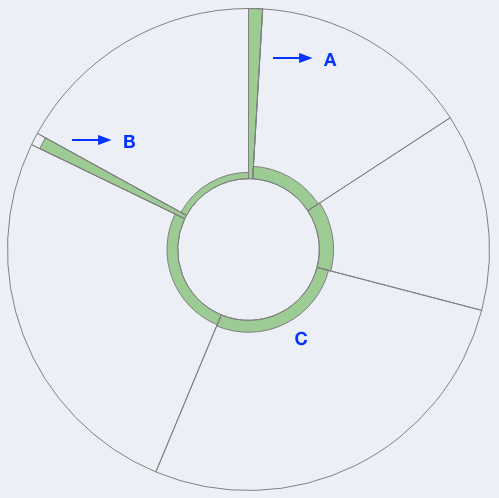
\includegraphics[scale=0.42]{Imagens/avaliacao_sumarizacao_otimizacao.png}}
   \textsf{\caption[Jetty, 9.3.12/9.3.13.]{Jetty, 9.3.12/9.3.13.\label{fig:avaliacao-sumarizacao-otimizacao}}}
   \end{subfigure}%
   \begin{subfigure}{.5\textwidth}
   \centering
   \frame{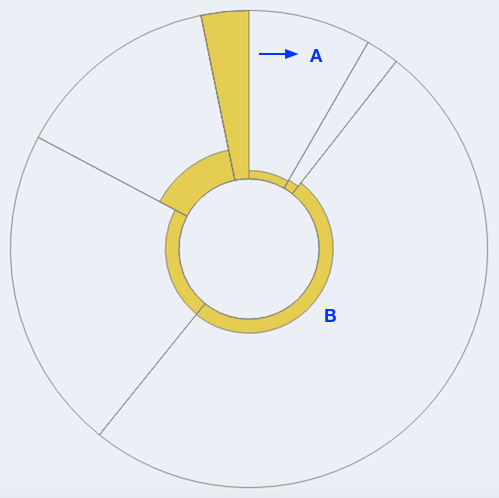
\includegraphics[scale=0.42]{Imagens/avaliacao_sumarizacao_degradacao.png}}
   \textsf{\caption[VRaptor, 4.2.0.RC2/4.2.0.RC3.]{VRaptor, 4.2.0.RC2/4.2.0.RC3.\label{fig:avaliacao-sumarizacao-degradacao}}}
   \end{subfigure}
   \begin{subfigure}{.5\textwidth}
   \centering
   \frame{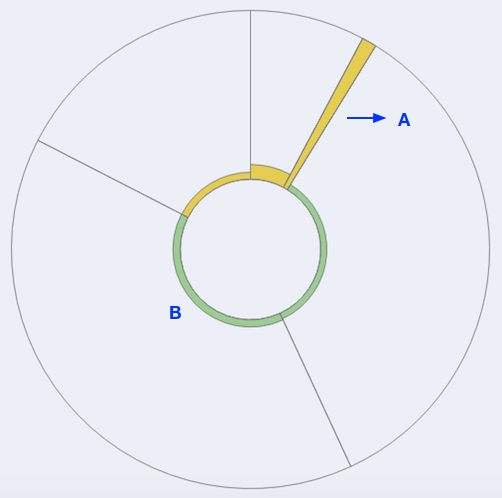
\includegraphics[scale=0.42]{Imagens/avaliacao_sumarizacao_misturado.png}}
   \textsf{\caption[Jetty, 9.3.14/9.3.15.]{Jetty, 9.3.14/9.3.15.\label{fig:avaliacao-sumarizacao-misturado}}}
   \end{subfigure}%
   \begin{subfigure}{.5\textwidth}
   \centering
   \frame{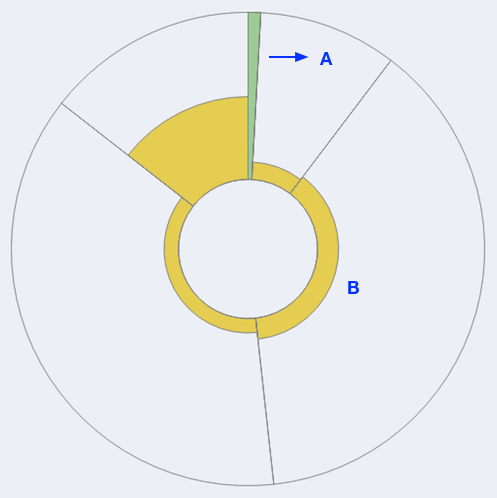
\includegraphics[scale=0.42]{Imagens/avaliacao_sumarizacao_misturado_2.png}}
   \textsf{\caption[VRaptor, 4.2.0.RC1/4.2.0.RC2.]{VRaptor, 4.2.0.RC1/4.2.0.RC2.\label{fig:avaliacao-sumarizacao-misturado-2}}}
   \end{subfigure}
   \caption{Exemplos da visualização de Sumarização de Cenários.}
  \label{fig:avaliacao-sumarizacao-exemplos-sucesso}
\end{figure}

\noindent\textbf{Visualização com Prejuízos}

Houve casos em que a identificação dos cenários na visualização pode ser prejudicada, de maneira geral: quando há muitos cenários com desvios de desempenho para o par de versões analisados. Quando isso acontece, as fatias ficam pequenas, dificultando a visualização, a localização pelo mouse e o clique para a visualização do grafo de chamadas. Em alguns casos, parte dos cenários apresentados podem ficar até mesmo ilegíveis. A figura \ref{fig:avaliacao-sumarizacao-ruim} apresenta esses casos.

\begin{figure}[!htb]
  \centering
   \begin{subfigure}{.5\textwidth}
   \centering
   \frame{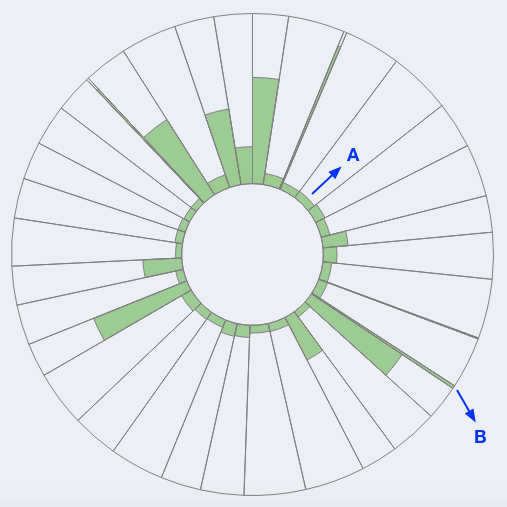
\includegraphics[scale=0.42]{Imagens/avaliacao_sumarizacao_ruim_1.png}}
   \textsf{\caption[Jetty, 9.3.11/9.3.12.]{Jetty, 9.3.11/9.3.12.\label{fig:avaliacao-sumarizacao-ruim-1}}}
   \end{subfigure}%
   \begin{subfigure}{.5\textwidth}
   \centering
   \frame{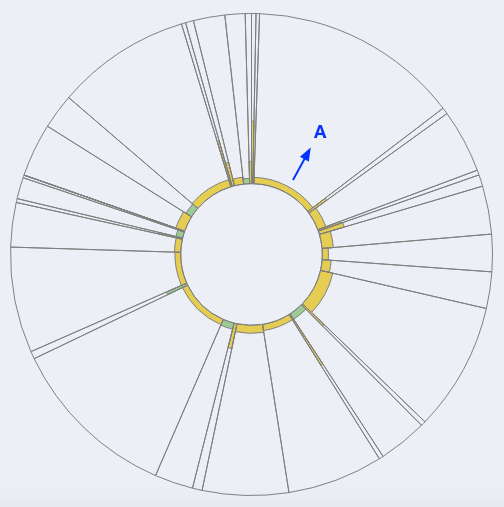
\includegraphics[scale=0.42]{Imagens/avaliacao_sumarizacao_ruim_2.png}}
   \textsf{\caption[Jetty, 9.3.16/9.4.0.]{Jetty, 9.3.16/9.4.0.\label{fig:avaliacao-sumarizacao-ruim-2}}}
   \end{subfigure}
   \begin{subfigure}{.5\textwidth}
   \centering
   \frame{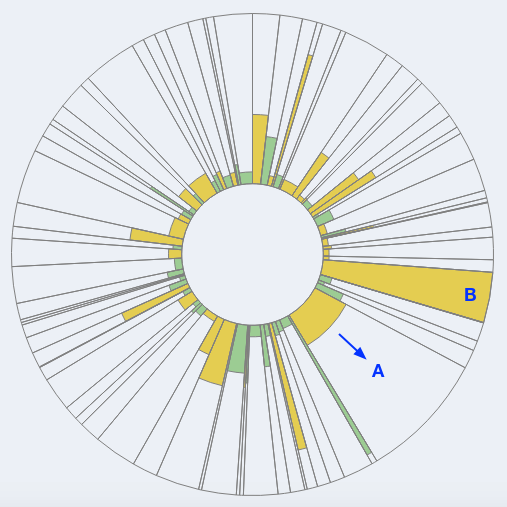
\includegraphics[scale=0.42]{Imagens/avaliacao_sumarizacao_ruim_3.png}}
   \textsf{\caption[VRaptor, 4.0.0.Final/4.1.0.Final.]{VRaptor, 4.0.0.Final/4.1.0.Final.\label{fig:avaliacao-sumarizacao-ruim-3}}}
   \end{subfigure}%
   \begin{subfigure}{.5\textwidth}
   \centering
   \frame{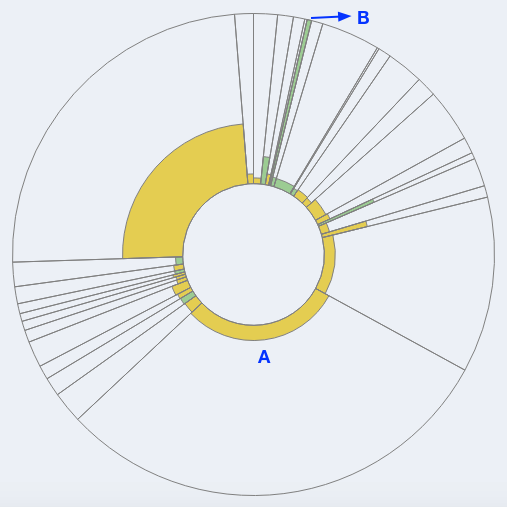
\includegraphics[scale=0.42]{Imagens/avaliacao_sumarizacao_ruim_4.png}}
   \textsf{\caption[VRaptor, 4.1.1/4.1.2.]{VRaptor, 4.2.0.RC1/4.2.0.RC2.\label{fig:avaliacao-sumarizacao-ruim-4}}}
   \end{subfigure}
   \caption{Exemplos da visualização de Sumarização de Cenários com excesso de cenários.}
  \label{fig:avaliacao-sumarizacao-ruim}
\end{figure}

Na figura \ref{fig:avaliacao-sumarizacao-ruim-1} são mostrados 36 cenários de otimização para o sistema \texttt{Jetty}, versões \texttt{9.3.11} para \texttt{9.3.12}. Nesse caso, os cenários estão com larguras distribuidas uniformemente, exceto 4 deles que tiveram baixa porcentagem de desvio e, portanto, suas fatias estão finas com relação às demais. Por causa dessa distribuição, pode ser complexo localizar o cenário \texttt{A}, que foi o que possuiu o maior porcentagem de desvio de desempenho (87,64\%). Nesse caso, como a distinção visual é difícil, é necessário passar o ponteiro do mouse sobre as fatias com largura semelhante para, somente após diferenciar os valores das porcentagens, constatar que o cenário \texttt{A} é o com maior desvio. O cenário \texttt{B} possuiu o maior tempo de execução. Sua identificação é menos difícil do que o cenário \texttt{A} pelo fato de existirem poucas fatias do gráfico com a mesma largura. Entretanto, o baixo desvio torna a fatia que representa esse cenário bastante fina, prejudicando a sua identificação visual.

A figura \ref{fig:avaliacao-sumarizacao-ruim-2} apresenta 34 cenários para o sistema \texttt{Jetty}, versões \texttt{9.3.16} para \texttt{9.4.0}. Nesse caso, embora a quantidade de cenários seja ligeiramente menor do que no caso anterior, a distribuição irregular ocasionada por diferentes porcentagens de desvios faz com que o cenário indicado pela letra \texttt{A} seja, através da distinção visual de sua largura perante os demais cenários, identificado como o cenário com maior desvio de desempenho (136,88\% de degradação) dentre os apresentados. Por outro lado, essa distribuição irregular fez com que o cenário com menor desvio de desempenho ficasse imperceptível na visualização: foram apenas 0,07\% de degradação. Coincidentemente, nesse caso, esse cenário é o que possui o maior tempo de execução dentre os exibidos e, através dessa visualização, não foi possível identificá-lo.

De todas as versões analisadas para os dois sistemas, as versões \texttt{4.0.0.Final} para \texttt{4.1.0.Final}, do sistema VRaptor, foi a que possuiu a maior quantidade de cenários identificados com desvios de desempenho: 77. A figura \ref{fig:avaliacao-sumarizacao-ruim-3} mostra a sumarização de cenários para esse caso. A distribuição irregular faz com que o cenário indicado com a letra \texttt{A} seja identificado como o que teve o maior desvio de desempenho (323,44\% de degradação), também, como no caso anterior, através da diferenciação visual das larguras das fatias. O cenário da letra \texttt{B} foi o que possuiu o maior tempo de execução e, como também teve uma porcentagem de degradação alta (127,27\%) comparado com a maioria dos cenários, sua identificação pode ser feita também por distinção visual. Embora a maioria dos cenários esteja legível por terem porcentagens de desvios de desempenho razoáveis, os que possuem baixa porcentagem de desvio podem ser difícieis de identificar.

A figura \ref{fig:avaliacao-sumarizacao-ruim-4} apresenta 30 cenários para o \texttt{VRaptor}, versões \texttt{4.2.0.RC1} para \texttt{4.2.0.RC2}. Através de diferenciação visual das larguras das fatias, como no caso anterior, o cenário da letra \texttt{A} pode ser identificado como o cenário que possuiu o maior desvio de desempenho: uma degradação de 730,93\%. De identificação mais difícil e não tão imediata como o cenário \texttt{A}, o cenário da letra \texttt{B} se apresenta como o de maior tempo de execução, porém com baixa porcentagem de desvio. Assim como no caso anterior, os cenários com baixa porcentagem de desvio de desempenho podem ser difíceis de identificar. No entanto, como nos casos da figura \ref{fig:avaliacao-sumarizacao-ruim-1} e \ref{fig:avaliacao-sumarizacao-ruim-3}, tanto o cenário com maior desvio de desempenho quanto o cenário com maior tempo de execução podem ser identificados.

Essa dificuldade em localizar os cenários, nesses casos, não necessariamente está ligada somente a quantidade de cenários apresentados pela visualização, mas também a distribuição das porcentagens de desvio. Quando há uma vasta quantidade de cenários a serem exibidos (acima de 15) e cenários com baixas porcentagens de desvio com relação aos demais, a identificação destes pode ser prejudicada.

Para resolver ou minimizar essa situação, podem ser feitas adaptações na implementação dessa visualização: (i) os cenários poderiam ser agrupados em módulos do sistema, de acordo com critérios definidos pelos usuários. Dessa forma, várias visualizações de sumarização de cenários seriam geradas, uma para cada módulo, e a ferramenta as apresentaria, uma a uma, com mecanismos de paginação entre os módulos; (ii) outra forma seria fazer um ranqueamento das maiores porcentagens de desvios de desempenho e agrupá-los por esse critério. Assim, utilizando um mecanismo de paginação para apresentá-las, na primeira página estariam os \textit{n} (por exemplo, 10) cenários com maior porcentagem de desvio de desempenho, e assim por diante nas páginas seguintes.

\begin{framed}
  \noindent Para 10 de 15 visualizações de sumarização de cenários geradas houve eficácia na apresentação dos casos analisados, de modo que o usuário pode distinguir, sem prejuízos, entre os cenários com maior/menor desvio de desempenho, além de maior/menor tempo de execução. Em 5 das 15 visualizações, quando há uma grande quantidade de cenários a serem exibidos (acima de 15) e cenários com baixas porcentagens de desvio de desempenho com relação aos demais, a identificação dos cenários com maior/menor desvio de desempenho ou com maior/menor tempo de execução foi prejudicada ou inviabilizada.
\end{framed}

\subsubsection{Grafo de Chamadas} \label{subsec:avaliacao-comportamento-grafo-chamadas}

Cada um dos 244 cenários identificados com desvios de desempenho pela ferramenta possuem nós a serem dispostos na visualização do grafo de chamadas. Nesta subseção serão destacados o resultado do algoritmo de supressão dos nós exibidos, bem como serão comentados 8 casos especiais de grafos.

\paragraph{Algoritmo de Supressão de Nós Exibidos}

Com a execução do algoritmo de supressão de nós exibidos (explicado na seção \ref{par:capitulo3-visualizacao2-algoritmo-supressao-nos}) para cada grafo de chamada gerado pela ferramenta, a redução da quantidade de nós a serem mostrados foi importante, consequentemente, diminuindo a complexidade de se encontrar informações. O gráfico exibido na figura \ref{fig:boxplot-porcentagem} indica que em 75\% dos cenários analisados a redução de nós se deu entre 73,77\% e 99,83\% e a mediana de redução de nós considerando todos os cenários é de 90,26\%. Os \textit{outliers} desse gráfico indicam os casos em que a porcentagem de redução foi considerada baixa. Isso pode acontecer, por exemplo, em cenários com poucos nós no total, onde a redução de nós a serem exibidos é baixa ou até mesmo inexistente.

O gráfico da figura \ref{fig:boxplot-reducao-nos} reforça o resultado do algoritmo, mostrando a distribuição da quantidade de nós exibidos no grafo de chamadas para os cenários analisados. Nesse gráfico, em 75\% dos cenários a quantidade de nós exibidos é entre 2 e 16 e a mediana de exibição dos nós considerando todos os cenários é de 9,5, indicando a baixa complexidade do grafo, na maioria dos casos. Entretanto, embora na maioria dos cenários a quantidade de nós exibidos seja baixa, houve casos em que essa quantidade pode ser considerada alta, conforme indicado pelos \textit{outliers} do gráfico. Por exemplo, o caso com maior quantidade de nós no grafo foi o cenário \texttt{Entry point for DispatcherForwardTest.testQueryRetai-\\nedByForwardWithoutQuery}, do Jetty, versões 9.3.16 para 9.4.0. Nesse cenário são exibidos 92 nós de um total de 5.376. Nesse caso, apesar de a quantidade de nós seja alta e seja considerado um \textit{outlier} no gráfico da figura \ref{fig:boxplot-reducao-nos}, a porcentagem de redução foi de 98,29\%, indicando a eficiência do algoritmo.

\begin{figure}[!htb]
  \centering
   \begin{subfigure}{.5\textwidth}
   \centering
   \frame{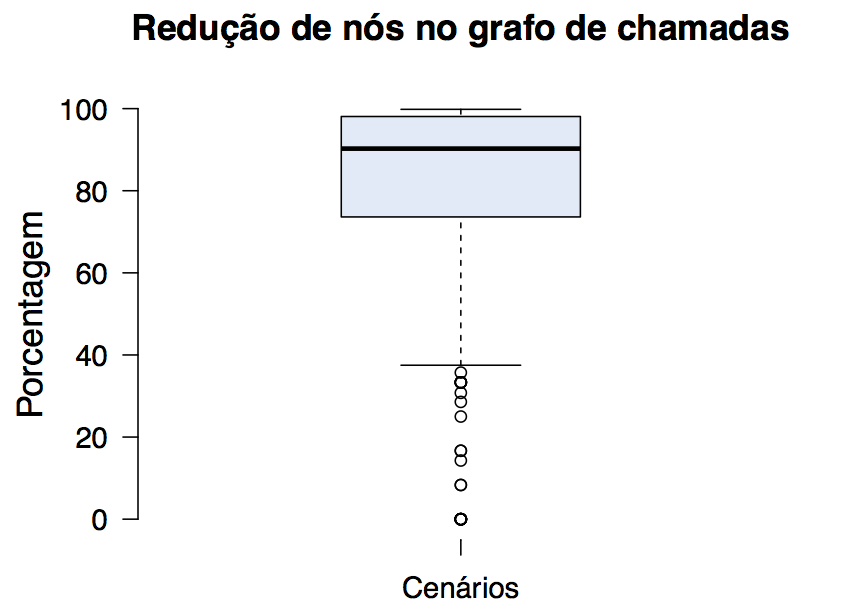
\includegraphics[scale=0.53]{Imagens/boxplot_porcentagem_reducao.png}}
   \textsf{\caption[Porcentagem de nós reduzidos.]{Porcentagem de nós reduzidos.\label{fig:boxplot-porcentagem}}}
   \end{subfigure}%
   \begin{subfigure}{.5\textwidth}
   \centering
   \frame{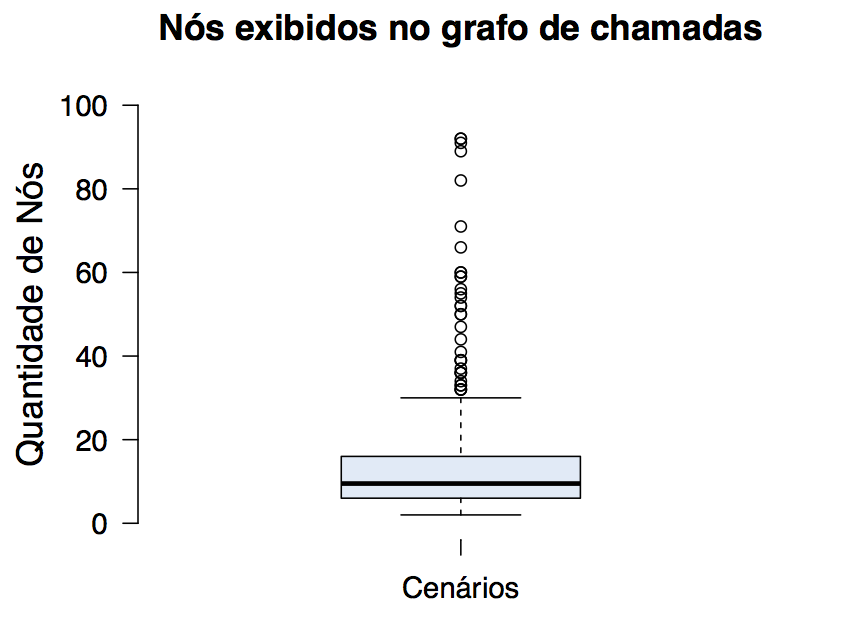
\includegraphics[scale=0.53]{Imagens/boxplot_nos_exibidos.png}}
   \textsf{\caption[Quantidade de nós exibidos.]{Quantidade de nós exibidos.\label{fig:boxplot-reducao-nos}}}
   \end{subfigure}
   \caption{Gráficos \textit{boxplot} sobre o algoritmo de redução de nós.}
  \label{fig:boxplot-porcentagem-reducao-nos}
\end{figure}

\begin{framed}
  \noindent O algoritmo de supressão de nós exibidos conseguiu reduzir, para 75\% dos cenários analisados, entre 73,77\% e 99,83\% a quantidade de nós a serem mostrados no grafo. Essa quantidade é de 2 a 16 nós exibidos, para 75\% dos cenários analisados.
\end{framed}

\paragraph{Casos Especiais}

Dentre os cenários analisados para os sistemas Jetty e VRaptor, alguns deles podem ser destacados por serem casos especiais de situações envolvendo a quantidade de nós degradados e otimizados, a porcentagem de redução dos nós exibidos e a porcentagem de desvio de desempenho de cenários. Os cenários que exemplificam esses casos são os seguintes:
\begin{itemize}
  \item \textit{Alta quantidade de nós degradados}: \texttt{Entry point for AsyncContextListeners-\\Test.testAsyncDispatchAsyncCompletePreservesListener} (C1)
  \item \textit{Alta quantidade de nós otimizados}:  \texttt{Entry point for ServletHolderTest.test-\\UnloadableClassName} (C2)
  \item \textit{Baixa porcentagem de redução de nós}: \texttt{Entry point for SafeResourceBundle-\\Test.shouldReturnKeyBetweenQuestionMarksWhenKeyDoesntExist} (C3)
  \item \textit{Alta porcentagem de redução de nós}: \texttt{Entry point for ServletContextHandler-\\Test.testInitOrder} (C4)
  \item \textit{Maior degradação}: \texttt{Entry point for DefaultEnvironmentTest.shouldUseCon-\\textInitParameterWhenSystemPropertiesIsntPresent} (C5)
  \item \textit{Menor degradação}: \texttt{Entry point for PostServletTest.testGoodPost} (C6)
  \item \textit{Maior otimização}: \texttt{Entry point for XStreamXmlDeserializerTest.shouldBe-\\AbleToDeserializeADogWhenMethodHasMoreThanOneArgumentAndTheXmlIsThe-\\LastOne} (C7)
  \item \textit{Menor otimização}: \texttt{Entry point for XStreamXMLSerializationTest.should-\\SerializeCollection} (C8)
\end{itemize}

A tabela \ref{tab:avaliacao-casos-especiais} a seguir resume alguns dados desses cenários. O cenário \texttt{C1} foi o cenário com a maior quantidade de nós degradados dentre os analisados: \texttt{10}. Houve também nós otimizados (\texttt{4}), adicionados (\texttt{10}) e removidos (\texttt{3}). Apesar de ter acontecido otimizações causadas pelos nós otimizados e removidos, o ganho de desempenho não foi suficiente para que o tempo total do cenário fosse otimizado. As degradações impostas pelos nós degradados e adicionados foram maiores, portanto, causando a degradação de \texttt{2,9\%}. Dentre as modificações que potencialmente causaram a degradação desse cenário, podem ser citados melhoramentos de tratamento de erros, permissão de personalização de métodos de classes, implementação de um conector para \textit{socket} e correção de cálculos para a verificação de número mínimos de \textit{threads} no servidor.

\begin{table}[!htb]
  \centering
  \textsf{\caption{Características dos cenários exemplos de casos especiais.\label{tab:avaliacao-casos-especiais}}}
  \medskip
  \resizebox{1.0\textwidth}{!}{
  \begin{tabular}{c|c|c|c|c|c|c|c}
    \textbf{Cenário} & \textbf{Sistema} & \textbf{Versão inicial/final} & \textbf{Tipo} & \textbf{\begin{tabular}[c]{@{}c@{}}\%\\Desvio\end{tabular}} & \textbf{\begin{tabular}[c]{@{}c@{}}Nós degradados/otimizados/\\adicionados/removidos\end{tabular}} & \textbf{\begin{tabular}[c]{@{}c@{}}Nós exibidos/\\total\end{tabular}} & \textbf{\begin{tabular}[c]{@{}c@{}}\%\\Redução\end{tabular}} \\ \hline
    C1 & Jetty & 9.3.16/9.4.0 & Degradação & 2,9 & 10/4/10/3 & 92/5.342 & 98,28 \\ \hline
    C2 & Jetty & 9.3.16/9.4.0 & Degradação & 4,07 & 1/8/6/3 & 71/718 & 90,11 \\ \hline
    C3 & VRaptor & 4.2.0.RC3/4.2.0.RC4 & Degradação & 124,49 & 1/0/0/0 & 2/2 & 0 \\ \hline
    C4 & Jetty & 9.3.11/9.3.12 & Otimização & 78,61 & 1/0/0/0 & 4/2.342 & 99,83 \\ \hline
    C5 & VRaptor & 4.2.0.RC3/4.2.0.RC4 & Degradação & 1.646 & 0/1/0/0 & 6/23 & 73,91 \\ \hline
    C6 & Jetty & 9.3.16/9.4.0 & Degradação & 0,07 & 0/0/5/0 & 28/98 & 71,43 \\ \hline
    C7 & VRaptor & 4.0.0.Final/4.1.0.Final & Otimização & 97,47 & 2/0/0/0 & 8/42 & 80,95 \\ \hline
    C8 & VRaptor & 4.1.2/4.1.3 & Otimização & 0,21 & 1/0/0/0 & 8/171 & 95,32 \\ \hline
  \end{tabular}
  }
\end{table}

O cenário C2 foi o cenário com a maior quantidade de nós otimizados: \texttt{8}. Assim como o cenário \texttt{C1}, também houve nós degradados (\texttt{1}), adicionados (\texttt{6}) e removidos (\texttt{3}). O resultado das otimizações e degradações impostas por esses nós foi um cenário degradado em \texttt{4,07\%}, apesar da alta quantidade de nós otimizados. Esses nós percentem a mesma classe do sistema: \texttt{Log}; e os métodos otimizados têm um baixo tempo de execução em nanosegundos. Diante disso, todas as \texttt{8} otimizações foram entre 0 e 25\% do tempo, fazendo com que os nós permanecessem, então, com um baixo tempo de execução. Por outro lado, os nós adicionados, alguns deles executando em loop, e o removido adicionaram tempos de execução suficientes para que o cenário se degradasse.

A menor porcentagem de redução de nós exibidos foi no cenário \texttt{C3}. A quantidade de nós exibidos é exatamente o total de nós que o cenário possui: \texttt{2}, sendo eles o nó raiz, que é o método da classe de teste automatizado que dá nome ao cenário, e o nó \texttt{SafeResourceBundle.handleGetObject(java.lang.String)}. O \textit{commit} que modificou este método indica uma mudança no mecanismo de \textit{log} que potencialmente é a causa da degradação de \texttt{124,49\%} do cenário. A figura \ref{fig:avaliacao-casos-especiais-c3} a seguir ilustra o grafo de chamadas do cenário \texttt{C3}.

\begin{figure}[!htb]
   \centering
   \frame{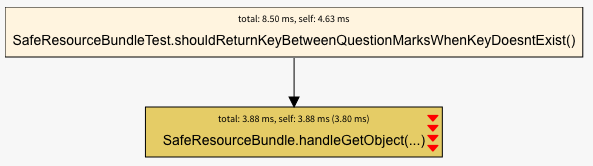
\includegraphics[scale=0.60]{Imagens/exemplo_casos_especiais_c3.png}}
   \textsf{\caption[Grafo de Chamadas do cenário \texttt{C3}.]{Grafo de Chamadas do cenário \texttt{C3}.\label{fig:avaliacao-casos-especiais-c3}}}
\end{figure}

A maior porcentagem de redução de nós exibidos se deu no cenário \texttt{C4}: \texttt{99,83\%}. De um total de \texttt{2.342} nós, são exibidos apenas \texttt{4}. Destes, um é o nó raiz que dá nome ao cenário, dois são nós agrupados, indicando a existência dos outros 2.338 nós, e o último é o nó que de fato houve desvio de desempenho, nesse caso, uma otimização. A figura \ref{fig:avaliacao-casos-especiais-c4} adiante exemplifica esse grafo.

\begin{figure}[!htb]
   \centering
   \frame{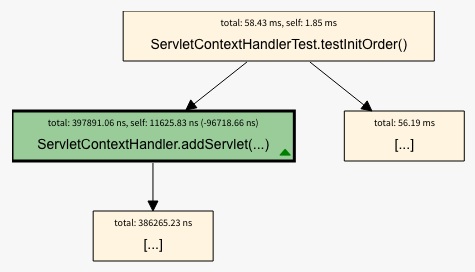
\includegraphics[scale=0.60]{Imagens/exemplo_casos_especiais_c4.png}}
   \textsf{\caption[Grafo de Chamadas do cenário \texttt{C4}.]{Grafo de Chamadas do cenário \texttt{C4}.\label{fig:avaliacao-casos-especiais-c4}}}
\end{figure}

O cenário \texttt{C5} foi o que mais degradou o seu tempo de execução em relação à versão anterior: \texttt{1.646\%}. O grafo da figura \ref{fig:avaliacao-casos-especiais-c5} mostra que o único nó com desvio de desempenho desse cenário apresentou uma degradação de mais de 75\%. O método representado por esse nó, \texttt{DefaultEnvironment.setup()}, é o responsável por prover uma implementação padrão que carrega o arquivo de ambiente com base na propriedades do sistema.

\begin{figure}[!htb]
   \centering
   \frame{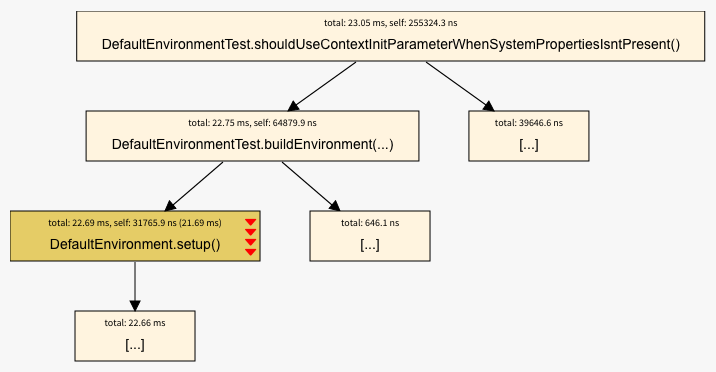
\includegraphics[scale=0.60]{Imagens/exemplo_casos_especiais_c5.png}}
   \textsf{\caption[Grafo de Chamadas do cenário \texttt{C5}.]{Grafo de Chamadas do cenário \texttt{C5}.\label{fig:avaliacao-casos-especiais-c5}}}
\end{figure}

O cenário que menos degradou dentre os analisados foi o \texttt{C6}: \texttt{0,07\%}. Cinco nós adicionados foram os responsáveis por essa degradação. No entanto, os seus tempos são pequenos (em nanosegundos) em comparação ao tempo do cenário (em segundos) e, por isso, a degradação causada por eles foi baixa. Em suma, as modificações impostas por esses nós adicionados são simples verificações com um \texttt{if}.

Outro caso especial que merece ser destacado é o cenário \texttt{C7}, que possuiu a com maior otimização dentre os analisados: \texttt{97,47\%}. Dois nós com otimizações de mais de \texttt{75\%} foram os responsáveis por esse desvio, adicionando uma estratégia recursiva para a configuração de um objeto da classe \texttt{com.thoughtworks.xstream.XStream}. A figura \ref{fig:avaliacao-casos-especiais-c7} exemplifica esse grafo.

\begin{figure}[!htb]
   \centering
   \frame{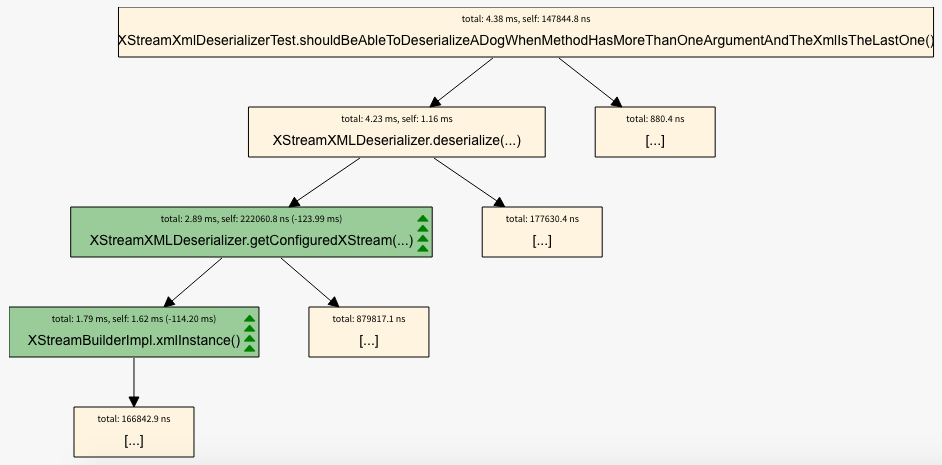
\includegraphics[scale=0.48]{Imagens/exemplo_casos_especiais_c7.png}}
   \textsf{\caption[Grafo de Chamadas do cenário \texttt{C7}.]{Grafo de Chamadas do cenário \texttt{C7}.\label{fig:avaliacao-casos-especiais-c7}}}
\end{figure}

O último cenário destacado é o \texttt{C8}, que possuiu a menor otimização. Como exibe o grafo da figura \ref{fig:avaliacao-casos-especiais-c8}, um único nó foi responsável por esse desvio, \texttt{XStreamBuilderImpl.xml-\\Instance()}. Esse nó teve uma otimização no seu desempenho de 0 a 25\% causada por uma mudança na chamada de um construtor. Isso fez com que o cenário otimizasse em apenas \texttt{0,21\%}.

\begin{figure}[!htb]
   \centering
   \frame{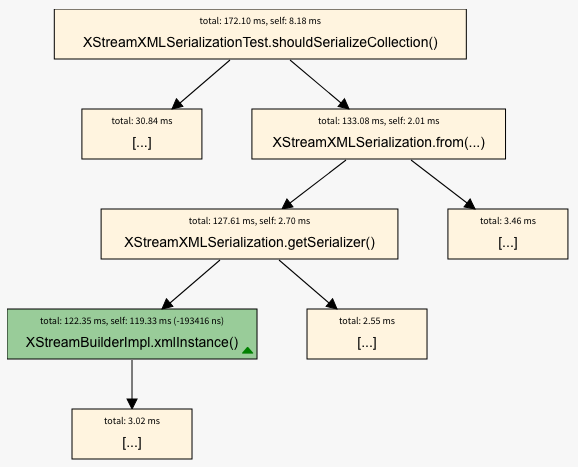
\includegraphics[scale=0.60]{Imagens/exemplo_casos_especiais_c8.png}}
   \textsf{\caption[Grafo de Chamadas do cenário \texttt{C8}.]{Grafo de Chamadas do cenário \texttt{C8}.\label{fig:avaliacao-casos-especiais-c8}}}
\end{figure}

A visualização do grafo de chamadas se mostrou eficaz na disposição dos nós dos cenários analisados. Através do grafo, é possível identificar os nós degradados, otimizados, adicionados e removidos, além de, através dos \textit{commits}, tomar conhecimento sobre as mudanças que potencialmente causaram esses desvios de desempenho.

\subsection{Questionário Online} \label{subsec:avaliacao-questionario-online}

O questionário online foi enviado para 114 contribuidores de ambos os sistemas. Desses, 16 responderam com algum feedback. Foram consideradas inválidas 3 dessas respostas, pelos motivos expostos na subseção \ref{subsec:avaliacao-caracterizacao-participantes}, restando, portanto, 13 respostas válidas. As respostas comentadas e expostas nesta subseção consideram apenas as respostas válidas.

\subsubsection{Grafo de Chamadas}

A seção do questionário sobre o grafo de chamadas foi respondida pelos 4 grupos: dois deles responderam o questionário do tipo 1 e os outros dois grupos responderam ao questionário de tipo 2. Nessa seção, foi perguntado se os usuários conseguiam identificar os possíveis métodos responsáveis pelo desvio de desempenho de determinado cenário, além de solicitar que os métodos fossem listados em dois grupos: otimizados e degradados. Dos 9 participantes que responderam a essa pergunta baseados na visualização (questionário tipo 1), 6 (67\%) deles responderam corretamente e um (11\%) respondeu parcialmente correto. Nesse caso, a resposta foi considerada parcialmente correta pois o participante não mencionou um dos métodos degradados. Por outro lado, dos 4 participantes que responderam à questão baseados em dados tabulares (questionário tipo 2), apenas um (25\%) respondeu corretamente. %A figura \ref{fig:avaliacao-questao-7-tipo-1} mostra as porcentagens das respostas para o questionário de tipo 1, e a figura \ref{fig:avaliacao-questao-7-tipo-2} para o questionário de tipo 2.

Em seguida, os participantes responderam à questão \textit{``Quão fácil foi responder à pergunta anterior?''}, para ambos os questionários. Considerando apenas os que responderam de maneira correta ou parcialmente correta, para o questionário em que os participantes responderam baseados na visualização, 4 (58\%) dos 7 acharam muito fácil ou fácil responder à questão comentada no parágrafo anterior. Por outro lado, o único participante que acertou a mesma questão baseado em dados tabulares achou fácil encontrar as informações solicitadas.

\begin{framed}
  \noindent Diante do exposto para as duas questões anteriores, pode-se obter indícios de que a visualização do grafo de chamadas se mostrou mais eficaz do que os dados tabulares (isto é, desconsiderando a existência dessa visualização) para se encontrar informações sobre os possíveis métodos responsáveis pelo desvio de desempenho de determinado cenário.
\end{framed}

% \begin{figure}[!htb]
%   \centering
%    \begin{subfigure}{.5\textwidth}
%    \centering
%    \frame{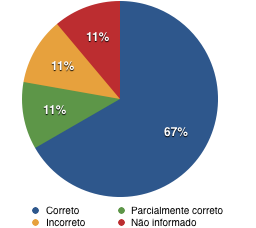
\includegraphics[scale=0.65]{Imagens/avaliacao_questao_7_tipo_1.png}}
%    \textsf{\caption[Questionário de tipo 1.]{Questionário de tipo 1.\label{fig:avaliacao-questao-7-tipo-1}}}
%    \end{subfigure}%
%    \begin{subfigure}{.5\textwidth}
%    \centering
%    \frame{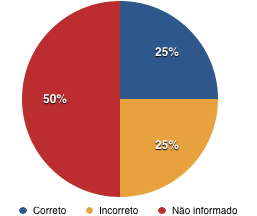
\includegraphics[scale=0.65]{Imagens/avaliacao_questao_7_tipo_2.png}}
%    \textsf{\caption[Questionário de tipo 2.]{Questionário de tipo 2.\label{fig:avaliacao-questao-7-tipo-2}}}
%    \end{subfigure}
%    \caption{Respostas dos participantes à questão para identificar os possíveis métodos responsáveis pelo desvio de desempenho de determinado cenário.}
%   \label{fig:avaliacao-questao-7}
% \end{figure}

Em seguida, uma questão, de ambos dos questionários, solicitou aos participantes que identificassem o \textit{hash} do \textit{commit} responsável por pelo principal desvio de desempenho do sistema. Dos 9 participantes que responderam a essa questão baseados na visualização do grafo de chamadas, 6 (67\%) deles acertaram a resposta. Por outro lado, dos 4 que responderam baseados nos dados tabulares, 2 (50\%) acertaram.

A próxima questão indagava \textit{``Quão fácil foi responder à pergunta anterior?''}, para ambos os questionários. Considerando apenas os 6 participantes que responderam corretamete à questão anterior no questionário de tipo 1, 5 (84\%) deles considerou muito fácil ou fácil. Por outro lado, para o questionário de tipo 2, dos 2 participantes que responderam à questão corretamente, apenas 1 (50\%) deles achou fácil.

\begin{framed}
  \noindent Tomando como base as respostas as duas perguntas anteriores, têm-se indícios de que a visualização do grafo de chamadas se mostrou novamente mais eficaz do que os dados tabulares para se encontrar os \textit{hashs} dos \textit{commits} responsáveis pelos principais desvios de desempenho do sistema.
\end{framed}

Através da visualização do grafo de chamadas, os participantes acessaram um cenário real a partir da execução da ferramenta em seus respectivos sistemas e tomaram conhecimento, se já não havia, sobre o desvio de desempenho deparado. Em resposta à pergunta \textit{``Este desvio parece plausível de acordo com o seu conhecimento do sistema?''}, 7 (54\%) dos 13 participantes com respostas válidas consideraram ser plausível o desvio de desempenho mostrado na visualização. Apenas 2 (15\%) responderam que não era plausível, enquanto que o restante não informou (3 - 28\%) ou não soube responder (1 - 8\%).

Na seção dos questionários de tipo 1 e 2 que tratavam das visualizações havia uma pergunta para os participantes relatarem as suas impressões: \textit{``Você poderia mencionar aspectos dessa visualização que você gostou? E quais outros aspectos você não gostou? Você tem alguma sugestão de melhoria ou comentário para essa visualização?''}. Para a visualização do Grafo de Chamadas, no geral, os participantes disseram gostar das características visuais implementadas, mas também fizeram críticas à visualização. O participante P5GA disse que \textit{``o gráfico é bastante simples e fácil de entender. Não há muita informação, apenas o necessário. Eu gostei do recurso de destaque e a seta verde/vermelha indicando o nível de melhoria/degradação. Como sugestão, pode ser interessante adicionar informações sobre o contexto de execução (ex: argumentos JVM)''}, já o participante P22GA menciona que \textit{``o popup Detalhes é difícil de copiar / colar. Eu preferiria que ele permanecesse aberto até eu clicar em outro lugar. Os links para o commit exato são agradáveis. Toda a visualização parece muito boa, mas gostaria que o grafo de chamadas tivesse um pouco mais de espaço em tela. Seria bom ter (temporariamente?) preenchendo a tela inteira. Por algum motivo, eu esperava poder clicar e arrastar o grafo de chamadas (como o Google Maps) em vez de usar a rolagem''}. O participante P13GC, no entanto, não percebeu que a funcionalidade de zoom foi implementada e relatou sentir falta: \textit{``gostei dos gráficos e dos detalhes das informações. Achei o espaço reservado para o grafo de chamadas muito reduzido, o espaço vertical pra ele é pequeno. Outra coisa que senti falta foi uma opção de Zoom Out no grafo de chamadas''}. O gráfico da figura \ref{fig:avaliacao-questao-12} quantifica as opiniões dos participantes com relação ao que gostaram, não gostaram ou as sugestões feitas por eles para essa visualização.

\begin{figure}[!htb]
   \centering
   \frame{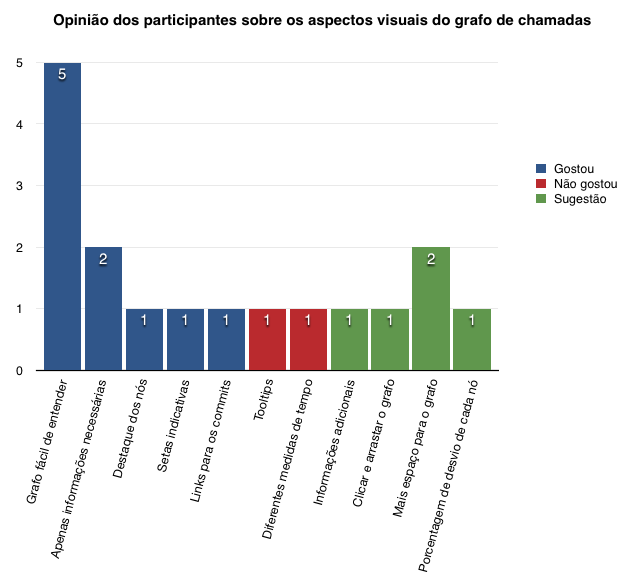
\includegraphics[scale=0.60]{Imagens/avaliacao_questao_12.png}}
   \textsf{\caption[Opinião dos participantes sobre os aspectos da visualização do grafo de chamadas.]{Opinião dos participantes sobre os aspectos da visualização do grafo de chamadas.\label{fig:avaliacao-questao-12}}}
\end{figure}

Dos aspectos que os participantes gostaram, é importante destacar que houve 5 opiniões de que o grafo está fácil de entender. Outras menções foram feitas para funcionalidades como a de destaque dos nós com desvio, as setas indicativas de nós degradados ou otimizados e os \textit{links} diretamente para os \textit{commits} que possívelmente foram os causadores do desvio de desempenho do referido nó.

Sobre os aspectos que os participantes não gostaram, o participante P22GA comentou sobre os \textit{tooltips}, conforme relatado no parágrafo anterior, e o participante P26GA mencionou que \textit{``as diferenças de unidades de tempo (ms, ns) podem atrapalhar as pessoas''}. Essa diferença das unidades de tempo foi implementada para que a quantidade de números exibidos nos nós seja a menor possível. Dessa forma, sempre que possível o tempo é convertido para a unidade superior. Por exemplo: um tempo de execução de 1.200.000 nanosegundos será automaticamente convertido para 1,2 milissegundos, já um tempo de 1.500 milissegundos será convertido para 1,5 segundos.

Como sugestões, o participante P5GA acha interessante visualizar informações sobre o contexto de execução do teste automatizado, como, por exemplo, os argumentos da JVM. Já o participante P22GA, em sua resposta, comentou que esperava poder clicar e arrastar o grafo para navegação. Diante dessa frustração, a implementação dessa funcionalidade foi colocada como sugestão. Dois participantes sugeriram mais espaço para o grafo de chamadas. Se possível, mesmo que temporariamente, exibi-lo em tela cheia. Por fim, outro participante acha interessante que haja a porcentagem de desvio de desempenho indicada nos nós.

\subsubsection{Sumarização de Cenários}

A seção do questionário sobre a sumarização de cenários também foi respondida pelos 4 grupos: dois deles responderam o questionário do tipo 1 e os outros dois grupos responderam o questionário de tipo 2. Foi perguntado se os participantes conseguiam identificar qual dos cenários, dadas duas versões de seus respectivos sistemas, possuiu o maior desvio de desempenho dentre os exibidos. Além disso, foi solicitado que eles indicassem se o cenário tinha sido otimizado ou degradado. Dos 4 participantes responderam a essa questão baseados na visualização da sumarização de cenários, 2 (50\%) a responderam corretamente e um (25\%) respondeu parcialmente correto. Nesse caso, a resposta foi considerada parcialmente correta pois o participante apenas apontou o nome do cenário, mas não se ele degradou ou otimizou. Por outro lado, dos que responderam baseados em dados tabulares, 5 (56\%) acertaram a resposta e uma (11\%) foi considerada parcialmente correta. A resposta foi considerada parcialmente correta, nesse caso, pois o participante não apontou o nome do cenário e se este degradou ou otimizou, ele apenas indicou em qual linha da tabela estava o cenário.

Em seguida, os participantes responderam à questão \textit{``Quão fácil foi responder à pergunta anterior?''} relacionada a questão do parágrafo anterior. Considerando apenas os participantes que responderam de maneira correta ou parcialmente correta a questão anterior, 2 (66\%) dos 3 que responderam baseados na visualização apontaram ser muito fácil ou fácil respondê-la. Já os participantes que responderam baseados em dados tabulares, 5 (88\%) dos 6 achou fácil ou muito fácil respondê-la.

\begin{framed}
  \noindent Diante do exposto para as duas questões anteriores, não há indícios suficientes para concluir se a visualização da sumarização de cenários traz ganhos na identificação dos cenários com maior desvio de desempenho dentre os exibidos, uma vez que o resultado foi semelhante com o uso de dados tabulares.
\end{framed}

Outra questão em que os participantes tinham que identificar um cenário a partir de suas características visuais foi para indicar o cenário com o maior tempo de execução dentre os exibidos, além de informar se ele foi otimizado ou degradado. Dois (50\%) participantes que responderam à questão baseados na visualização acertaram, além de um (25\%) que acertou parcialmente, de um total de 4. O participante que acertou parcialmente apenas informou o nome do cenário, mas não se este foi degradado ou otimizado. Por outro lado, dos que responderam baseados em dados tabulares, 5 (56\%) responderam corretamente e um (11\%) parcialmente correto. O participante que acertou parcialmente informou apenas a situação do cenário, porém não informou o seu nome.

Novamente, após a questão anterior, os participantes responderam à questão \textit{``Quão fácil foi responder à pergunta anterior?''}. Considerando apenas os participantes que responderam de maneira correta ou parcialmente correta a questão anterior, 2 (66\%) dos 3 que responderam baseados na visualização apontaram ser muito fácil ou fácil respondê-la. Os 6 participantes que responderam baseados nos dados tabulares acharam muito fácil ou fácil respondê-la.

\begin{framed}
  \noindent Para as duas questões anteriores, também não há indícios suficientes para concluir se a visualização da sumarização de cenários traz ganhos na identificação dos cenários com maior tempo de execução dentre os exibidos, uma vez que o resultado foi semelhante com o uso de dados tabulares.
\end{framed}

De maneira igual a seção dos questionários referentes a visualização do grafo de chamadas, os participantes responderam a questão \textit{``Você poderia mencionar aspectos dessa visualização que você gostou? E quais outros aspectos você não gostou? Você tem alguma sugestão de melhoria ou comentário para essa visualização?''}. O sentimento foi dividido. O participante P1GD não se sentiu confortável com o gráfico de rosca utilizado para a visualização: \textit{``gráficos em torta ou semelhantes normalmente querem representar 100\% de algo. Usar a largura versus altura não foi intuitivo pra mim. Talvez separar mesmo em dois gráficos e dar a opção de ordenar ou por um ou por outro}. Por outro lado, o participante P6GD gostou e comentou que \textit{``utilizar a largura, cor e altura da fatia me pareceu uma boa definição para identificação dos aspectos analisados''}.

\subsubsection{Questões Finais}

Após responderem sobre as visualizações, a seção final do questionário convidou os participantes a responderem a questões gerais sobre os benefícios, a utilidade da ferramenta além de comentários gerais. Na primeira das questões dessa seção, os participantes responderam a questão \textit{``Você vê benefícios de usar a ferramenta de visualização de desvios de desempenho apresentada? Se sim, quais?''}. Do total de participantes com respostas válidas, \texttt{9} (69\%) deles disseram que veem benefícios no uso da ferramenta, conforme exibe a figura \ref{fig:avaliacao-questao-17}. Dentre os benefícios comentados pelos participantes, o participante P8GC disse que \textit{``aparentemente pode trazer análises mais assertivas do atual desempenho do sistema''}, já o participante P13GC menciona que \textit{``sim, é bem interessante para verificar se os novos releases contém alterações com prejuízos sérios à performance, podendo algumas vezes até detectar algum problema de lógica ou regra de negócio''}, ao passo que o participante P6GD informa que \textit{``sim. É interessante saber de maneira precisa e quantitativa a quantidade e nível de melhorias e degradações entre versões''}.

Os \texttt{2} (15\%) que talvez vejam benefícios na ferramenta também merecem destaque. O participante P19GD respondeu que \textit{``Acho a idéia muito interessante, mas acredito que o projeto ainda precise evoluir bastante para se tornar usável.''}. Já o participante P11GA disse que se sente \textit{``duvidoso com relação a falsos positivos/negativos de testes automatizados que não foram projetados para serem comparados.''}.

\begin{figure}[!htb]
  \centering
  \begin{subfigure}{.50\textwidth}
   \centering
   \frame{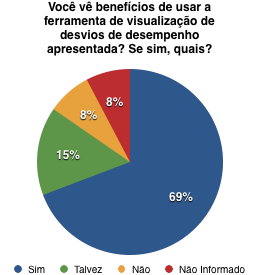
\includegraphics[scale=0.55]{Imagens/avaliacao_questao_17.png}}
   \textsf{\caption[Benefícios da ferramenta.]{Benefícios da ferramenta.\label{fig:avaliacao-questao-17}}}
   \end{subfigure}%
   \begin{subfigure}{.50\textwidth}
   \centering
   \frame{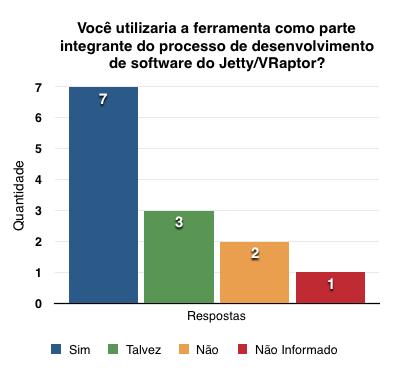
\includegraphics[scale=0.55]{Imagens/avaliacao_questao_18.png}}
   \textsf{\caption[Utilidade da ferramenta.]{Utilidade da ferramenta.\label{fig:avaliacao-questao-18}}}
   \end{subfigure}
   \caption{Questões sobre os benefícios e utilidade da ferramenta.}
  \label{fig:avaliacao-questoes-17-18}
\end{figure}

Com relação à questão \textit{``Você utilizaria a ferramenta como parte integrante do processo de desenvolvimento de software do Jetty/VRaptor? Se sim, como você vislumbra que ela seria utilizada?''}, \texttt{7} (54\%) dos participantes respondeu que usaria a ferramenta como parte integrante do processo de desenvolvimento. O participante P22GA disse que \textit{``eu imagino usar esta ferramenta de duas maneiras: monitoramento regular para ver como as mudanças afetam o desempenho e investigação focada em uma questão específica''}, já o participante P8GC reforça que \textit{``talvez ela pudesse fazer parte do conjunto de análises antes da release''}, o participante P13GC afirma que \textit{``Sim. Acho que poderia ser utilizada para avaliar releases antes de serem lançadas, para garantir que não há consequencias graves à performance após as evoluções implementadas''} e o participante P18GD disse que \textit{``sim. Integrada ao ciclo de entrega continua (acredito que usam travis.ci) para geração de reports (configurado no maven)''}. A figura \ref{fig:avaliacao-questao-18} sumariza as respostas à essa questão e expõe que a maioria dos usuários usariam a ferramenta em seus processos de desenvolvimento.

Vale destacar que \texttt{3} (23\%) responderam talvez à questão do parágrafo anterior. Dentre as justificativas apresentadas por eles, o participante P4GA disse que \textit{``não sei dizer. Não tenho certeza sobre outros testes mais complexos e de integração''}, já o participante P19GD comentou que \textit{``não neste momento. Posteriormente poderia fazer parte de uma análise de status do projeto antes de um release''}. Essas responstas indicam que, caso tivessem mais conhecimento e experiência sobre a ferramenta, eles são potenciais usuários a integrarem-na aos seus processos de desenvolvimento.

\begin{framed}
  \noindent Dos 13 participantes com respostas válidas, 9 (69\%) veem benefícios em se utilizar a ferramenta e 7 (54\%) usariam a ferramenta em seus processos de desenvolvimento de software.
\end{framed}

A última questão dos questionários convidou os participantes a deixar comentários gerais sobre a ferramenta. A maioria deles deixou comentários positivos, no entanto, houve críticas. O participante P1GD comentou: \textit{``achei algo bem profissional o que fizeram. Ainda está muito com cara de produto para hacker/coder, algo que já não sou mais, e fico perdido.''}. Já o participante P19GD comentou: \textit{``gostei da idéia do projeto, mas acho que precisa de alguns ajustes, principalmente na exibição das informações. Por exemplo, na planilha tem colunas em `ns', outras em `ms', mas que todas poderiam ter sido normalizadas para facilitar as comparações.''}. O participante P11GA disse \textit{``A análise é boa, mas o alvo ser testes unitários é pobre. Eu não me importo com o desempenho de 90\% dos casos de teste... Eles estão muitas vezes testando erros e mau comportamento.''}. Outro participante (P26GA) disse que \textit{``parece ótimo''}.

\section{Considerações} \label{sec:avaliacao-consideracoes}

Os resultados obtidos após a aplicação da ferramenta proposta mostram, de maneira geral, a sua utilidade ao prover aos desenvolvedores e arquitetos um ambiente para análise da evolução do atributo de qualidade de desempenho dos sistemas, sobretudo a visualização do grafo de chamadas. Os objetivos do estudo {\color{red} continuar...}
A ferramenta foi capaz de mostrar visualmente a evolução do desempenho dos cenários para o Jetty e VRaptor, além de apontar quais os métodos, e seus \textit{commits}, foram os possíveis causadores de tal desvio. Além disso, através do feedback obtido após a aplicação do questionário, os participantes relataram que vêem benefícios ao se utilizar a ferramenta e que ela pode ser integrada ao processo de desenvolvimento de software.

A expectativa, através dos resultados desse estudo, é ajudar os desenvolvedores e arquitetos a analisar o desempenho dos sistemas, facilitando a correção de gargalos de desempenho, através da identificação das suas causas, inseridos durante o desenvolvimento de determinada release. Dessa forma, integrada ao processo de desenvolvimento de software, a ferramenta pode ser usada de maneira preventiva, evitando a liberação de releases com problemas de desempenho desconhecidos. Embora nem toda degradação de desempenho seja passível de correção (por exemplo, a inserção de verificações de segurança de maneira planejada), a ferramenta provê a possibilidade de acompanhá-las.

Assim, as principais contribuições são: (i) a identificação visual dos cenários que mais tiveram desvios de desempenho para os sistemas Jetty e VRaptor, a partir da análise de múltiplas releases; (ii) a identificação visual dos cenários com maior tempo de execução para os sistemas analisados; (iii) para os mesmos sistemas, a percepção visual do tipo de desvio dos cenários através da análise de múltiplas releases; (iv) a distinção visual dos nós que tiveram desvio de desempenho (degradação ou otimização), foram adicionados ou removidos para cada cenário dos sistemas analisados; (v) para cada um desses nós, a indicação das potenciais causas dos desvios de desempenho, adição ou remoção ocorridos; ... {\color{red} continuar...} O restante desta seção comenta algumas limitações e ameaças a validade do estudo.

\subsection{Medição do Desempenho}

O \textit{\perfMinerName} se baseia em múltiplas execuções dos cenários para aumentar a confiança das medidas dos tempos de execução. Nesse estudo, todos os cenários foram executados 10 vezes para a análise do desvio de desempenho, mesmo assim alguns métodos em particular podem ter sido executados mais vezes. Por exemplo, os métodos podem ter várias hierarquias de chamadas, podem ser chamados em loops, etc. Para diminuir os riscos de viés na medição dos tempos de execução, foram tomadas precauções como desabilitar os serviços não essenciais do sistema operacional, cada teste foi executado em uma sua própria JVM e cada teste foi executado em ordem randômica \cite{Pinto2015}.

\subsection{Testes Unitários} \label{subsec:avaliacao-consideracoes-testes-unitarios}

Um dos participantes (P11GA) que respondeu ao questionário online aplicado mostrou preocupação sobre a utilização de testes unitários na análise. Segundo o participante, o atributo de qualidade de desempenho não é importante para 90\% dos testes unitários do sistema dele, pois eles apenas testam erros e mau comportamento. O \textit{\perfMinerName} utiliza esses casos de testes para a análise dos cenários, no entanto, quaisquer estratégias utilizadas para exercitar os cenários são válidas, pois a ferramenta continuará apontando os cenários com desvios de desempenho para os sistemas analisados. Como trabalho futuro, há a expectativa de que a ferramenta forneça a possibilidade de configurações dos cenários desejados para que os usuários escolham, de maneira não intrusiva, os cenários em que o desempenho é importante de acordo com as regras de negócio dos seus sistemas.

\subsection{Falsos Negativos e Falsos Positivos}

Quando da medição dos tempos de execução dos métodos, o \textit{\perfMinerName} identifica os cenários com desvios de desempenho usando média aritmética ou estratégias de testes estatísticos \cite{Pinto2015}. Com todos os casos de desvios definidos, a ferramenta realiza a mineração dos \textit{commits}. A ferramenta não sofre de falsos negativos uma vez que cada \textit{commit} está relacionado a um método com desvio (quando a causa do desvio é um elemento de código). Não há a possibilidade de, por exemplo, a ferramenta indicar um desvio de desempenho ocorrido por uma mudança de configuração ou por mudanças de infraestrutura, uma vez que não existirão códigos-fonte relacionados.

No entanto, falsos positivos podem acontecer porque diferentes \textit{commits} podem afetar o mesmo artefato de código-fonte durante uma evolução, ou pelo fato de um método ter sido impactado por outro método que também foi modificado durante a mesma evolução. Para resolver esse problema, pode ser adotada uma estratégia de análise por \textit{commit}, ao invés de por release \cite{Pinto2015}.

\subsection{Dados Tabulares}

Os questionários elaborados para o estudo foram de dois tipos, conforme destacado na subseção \ref{subsec:avaliacao-procedimentos-passo-3}: tipo 1 e tipo 2. Em ambos, os participantes responderam a questões relacionadas a uma visualização através da ferramenta proposta e a outra visualização através dos dados tabulares, isto é, sem ter acesso à visualização. Essa estratégia foi adotada para que se pudesse obter evidências da eficácia das visualizaçãoes, analisando as respostas dos dois tipos de questionários. Os dados tabulares utilizados são fruto do processamento feito pelo \textit{\perfMinerName}, portanto, são dados já pré-processados. Dessa forma, mesmo sem o acesso à visualização, os participantes conseguiram responder às questões de maneira razoável.

\subsection{Generalização e Limitação dos Resultados}

Os resultados encontrados neste estudo não podem ser generalizados. Com relação ao domínio e quantidade de sistemas analisados, a ferramenta foi aplicada apenas a dois sistemas de domínios diferentes. Para outros domínios e sistemas com outras características, não há evidências de que as visualizações sejam geradas corretamente, tampouco que sejam úteis às equipes de desenvolvimento desses sistemas. Outro fator limitativo é a quantidade de participantes do questionário online, sobretudo a quantidade de feedback obtido. Além disso, a quantidade de respostas do questionário de tipo 1 foi maior do que o de tipo 2, fornecendo maior feedback para a visualização do grafo de chamadas do que para a sumarização de cenários. Embora os resultados encontrados não possam ser generalizados, há evidências de que a ferramenta é útil para uma equipe de desenvolvimento e traz informações importantes sobre o desempenho dos sistemas.